%! Author = lazza
%! Date = 28/05/2022

\section{GPU}\label{sec:gpu}

\subsection{Procedural synthesis}\label{subsec:procedural-synthesis}
Procedural synthesis about making optimal use of system bandwidth
and main memory by dynamically generating lower-level geometry
data from statically stored higher-level scene data.

\begin{figure}[h]
    \centering
    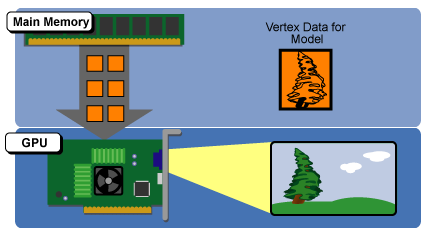
\includegraphics[width = \linewidth]{images/procedural-synthesis}
    \caption{Procedural synthesis}
    \label{fig:procedural-synthesis}
\end{figure}

For 3D games:
\begin{itemize}
    \item Artists use a 3D rendering program to produce content for the game
    \item Each model is translated into a collection of polygons
    \item Each polygons is represented in the computer's memory as collections of vertices
\end{itemize}
When the computer is rendering a scene in a game in real-time:
\begin{itemize}
    \item Models that are being displayed on the screen start out in main
memory as stored vertex data
    \item That vertex data is fed from main memory into the GPU where it is then rendered into a 3D image and output
    to the monitor as a sequence of frames.
\end{itemize}

\paragraph{Limitations} there are two problems:
\begin{itemize}
    \item The costs of creating art assets for a 3D game are
going through the roof along with the size and
complexity of the games themselves
    \item Console hardware's limited main memory sizes and
limited bus bandwidth
\end{itemize}

\paragraph{Xbox 360's solution}
Store high-level descriptions of objects in main memory.
Give the CPU the task of procedurally generate the geometry of the objects on the fly -- e.g., the vertex data are
generated by one or more running threads.
The GPU then takes the pre-processed vertex information and renders the tress normally, just as if it had gotten that
information from main memory.

\begin{figure}[h]
    \centering
    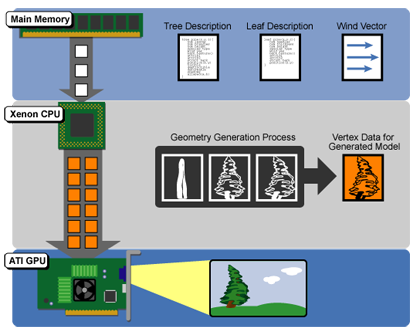
\includegraphics[width=\linewidth]{images/xbox-360-image-processing}
    \caption{Xbox 360 image processing}
    \label{fig:xbox-360-image-processing}
\end{figure}

\subsection{GPU vs CPU}\label{subsec:gpu-vs-cpu}
A GPU is tailored for high parallel operation while a
CPU executes programs serially.
For this reason, GPUs have many parallel execution
units and higher transistor counts, while CPUs have few
execution units and higher clock speeds.
A GPU is for the most part deterministic in its operation
(though this is quickly changing).
GPUs have much deeper pipelines (several thousand
stages vs 10--20 for CPUs).
GPUs have significantly faster and more advanced
memory interfaces as they need to shift around a lot
more data than CPUs.

\subsection{GPU pipeline}\label{subsec:gpu-pipeline}
The GPU receives geometry information from the CPU as an input and provides a picture as an output.
The five stages are:
\begin{itemize}
    \item host interface
    \item vertex processing
    \item triangle setup
    \item pixel processing
    \item memory interface
\end{itemize}

\begin{figure}[h]
    \centering
    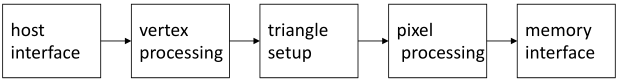
\includegraphics[width=\linewidth]{images/gpu-pipeline}
    \caption{GPU pipeline}
    \label{fig:gpu-pipeline}
\end{figure}

\subsubsection{Host interface}
The host interface is the communication bridge between the CPU and the GPU\@.
It receives commands from the CPU and also pulls geometry information from system memory.
It outputs a stream of vertices in object space with all their associated information (normals, texture
coordinates, per vertex color, etc.)

\subsubsection{Vertex processing}
The vertex processing stage receives vertices from the host interface in object space and outputs them in screen space.
This may be a simple linear transformation, or a complex operation involving morphing effects.
Normals, texcoords, etc., are also transformed.
No new vertices are created in this stage, and no vertices are discarded (input/output has 1:1 mapping).

\subsubsection{Triangle setup}
In this stage geometry information becomes raster information: screen space geometry is the input, pixels are the 
output.
Prior to rasterization, triangles that are back-facing or are located outside the viewing frustum are rejected.
Some GPUs also do some hidden surface removal at this stage.

\subsubsection{Fragment processing}
Each fragment provided by triangle setup is fed into fragment processing as a set of attributes (position, normal, 
textcoord, etc.), which are used to compute the final color for this pixel.
The computation taking place here include texture mapping and math operations.
Typically the bottleneck in modern applications.

\subsubsection{Memory interface}
Fragment colors provided by the previous stage are written to the framebuffer.
It used to be the biggest bottleneck before fragment processing took over.
Before final write occurs, some fragments are rejected by the zbuffer, stencil and alpha tests.
On modern GPUs, z and color are compressed to reduce framebuffer bandwidth (but not size).


\subsection{Programmability in the GPU}\label{subsec:programmability-in-the-gpu}
Vertex and fragment processing, and now triangle set-up, are programmable.
The programmer can write programs that are executed for every vertex as well as for every fragment.
This allows fully customizable geometry and shading effects that go well beyond the generic look and feel of old 3D
applications.

\begin{figure}[h]
    \centering
    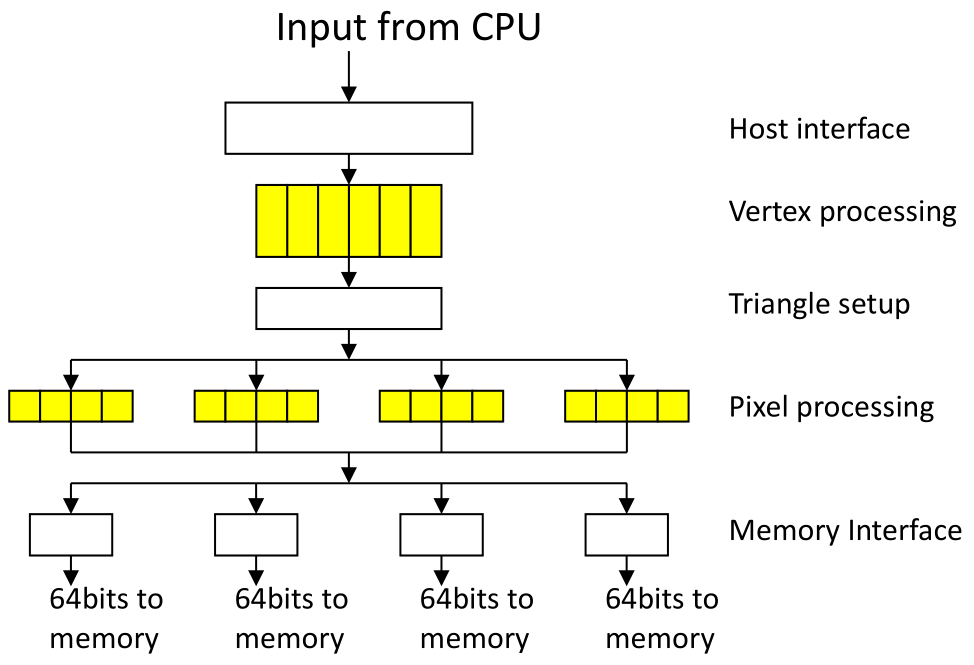
\includegraphics[width=\linewidth]{images/gpu-hierarchy}
    \caption{GPU pipeline}
    \label{fig:gpu-hierarchy}
\end{figure}

\subsection{Command buffer CPU-GPU}\label{subsec:command-buffer-cpu-gpu}
The CPU and GPU inside the \textit{heterogeneous} system work in parallel with each other.
There are two "threads" going on, one for the CPU and one for the GPU, which communicate through a command buffer:

\begin{figure}[h]
    \centering
    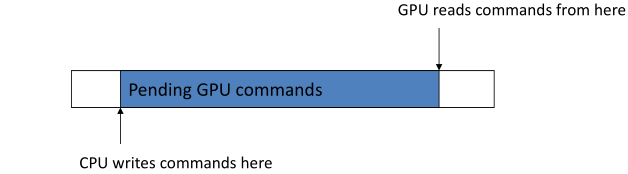
\includegraphics[width=\linewidth]{images/gpu-command-buffer}
    \caption{GPU command buffer}
    \label{fig:gpu-command-buffer}
\end{figure}

If this command buffer is drained empty, we are CPU limited and the GPU will spin around waiting for new input.
If the command buffer fills up, the CPU will spin around waiting for the GPU to consume it, and we are effectively
GPU limited.

Another important point to consider is that programs that use the GPU do not follow the traditional sequential
execution model.
In the CPU program below, the object is not drawn after statement A and before statement B:
\begin{center}
    \textbf{statement A}\\
    \textcolor{red}{\textbf{API call to draw object}}\\
    \textbf{statement B}
\end{center}

Instead, all the API call does, is to add the command to draw the object to the GPU command buffer.

\subsubsection{Synchronization issues}
\paragraph{Referring data}
In figure~\ref{fig:gpu-buffer-referring-data}, the CPU must not overwrite the data in the "yellow" block until the GPU
is done with the "black" command, which references that data.

\begin{figure}[h]
    \centering
    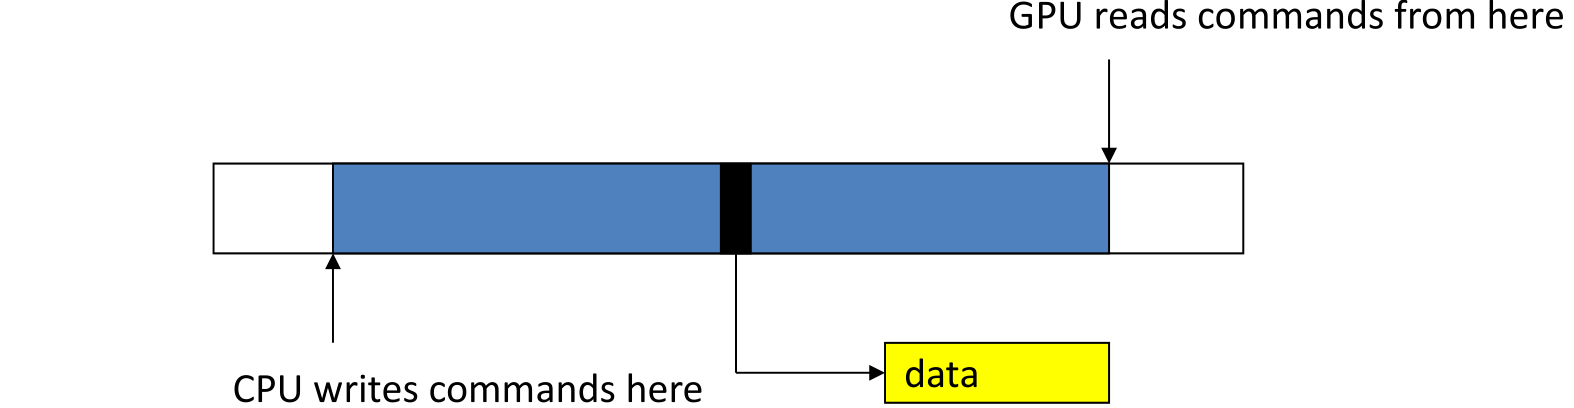
\includegraphics[width=\linewidth]{images/gpu-buffer-referring-data}
    \caption{Referring data}
    \label{fig:gpu-buffer-referring-data}
\end{figure}

Moderns APIs implement semaphore style operations to keep this from causing problems.
If the CPU attempts to modify a piece of data that is being referenced by a pending GPU command it will have to spin
around waiting, until the GPU is finished with that command.
While this ensures correct operation it is not good for
performance since there are a million other things we’d
rather do with the CPU instead of spinning.
The GPU will also drain a big part of the command
buffer thereby reducing its ability to run in parallel with
the CPU\@.

\paragraph{Inlining data}
One way to avoid these issues is to inline all data to the command buffer and avoid references to separate data:

\begin{figure}[h]
    \centering
    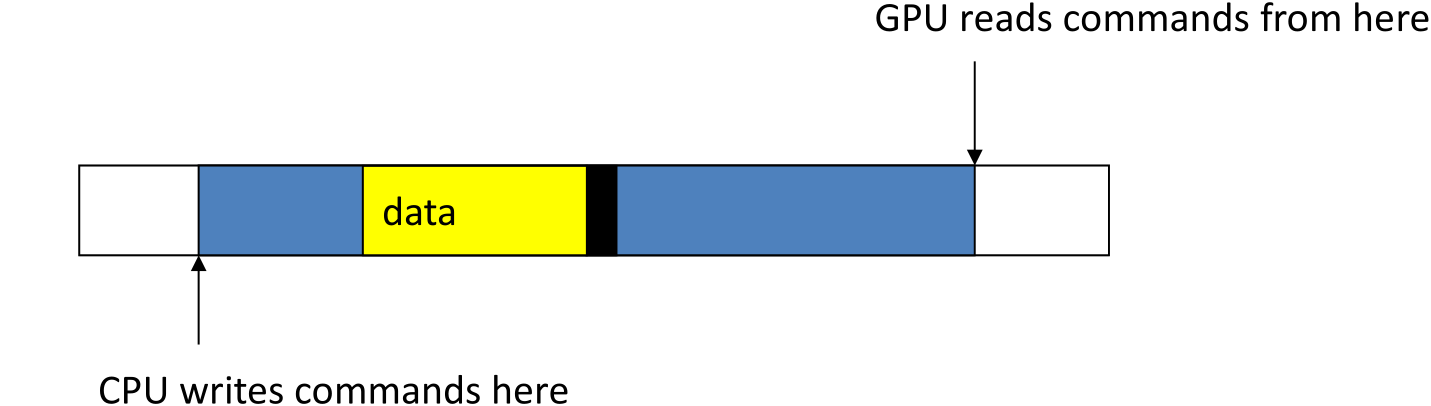
\includegraphics[width=\linewidth]{images/gpu-buffer-inlining-data}
    \caption{Inlining data}
    \label{fig:inlining-data}
\end{figure}

However, this is also bad for performance, since we
may need to copy several megabytes of data instead of
merely passing around a pointer.

\paragraph{Renaming data}
A better solution is to allocate a new data block and
initialize that one instead, the old block will be deleted
once the GPU is done with it.
Modern APIs do this automatically, provided you
initialize the entire block (if you only change a part of the
block, renaming cannot occur).

\begin{figure}[h]
    \centering
    
\includegraphics[width=\linewidth]{images/gpu-buffer-renaming-data}
    \caption{Renaming data}
    \label{fig:gpu-buffer-renaming-data}
\end{figure}

Better yet, allocate all your data at startup and don’t
change them for the duration of execution (not always
possible, however).

\subsubsection{GPU read-backs}
The output of a GPU is a rendered image on the screen,
what will happen if the CPU tries to read it?
The GPU must be synchronized with the CPU, i.e., it
must drain its entire command buffer, and the CPU must
wait while this happens.
We lose all parallelism, since first the CPU waits for the
GPU, then the GPU waits for the CPU (because the
command buffer has been drained).
Both CPU and GPU performance take a nosedive.
\textbf{Bottom line:} the image the GPU produces is for your
eyes, not for the CPU (treat the CPU \textrightarrow GPU highway as
a one way street).

\subsubsection{GPU tips}
Since the GPU is highly parallel and deeply pipelined,
try to dispatch large batches with each drawing call.
Sending just one triangle at a time will not occupy all of
the GPU’s several vertex/pixel processors, nor will it fill
its deep pipelines.

Since all GPUs today use the zbuffer algorithm to do
hidden surface removal, rendering objects front-to-back
is faster than back-to-front (painters algorithm), or
random ordering.
Of course, there is no point in front-to-back sorting if you
are already CPU limited.

\paragraph{nVidea G80 GPU} Characteristics:\\
\textrightarrow 128 streaming floating point processors @1.5Ghz\\
\textrightarrow 1.5 Gb Shared RAM with 86Gb/s bandwidth\\
\textrightarrow 500 GFLOPS on one chip (single precision)

\begin{figure}[h]
    \centering
    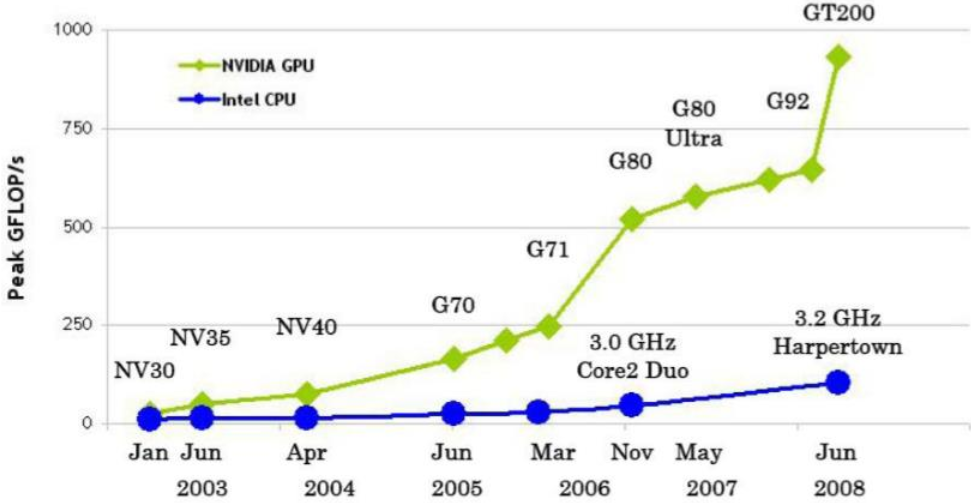
\includegraphics[width=\linewidth]{images/cpu-vs-gpu-performance}
    \caption{CPU vs GPU comparison}
    \label{fig:cpu-vs-gpu-performance}
\end{figure}

\paragraph{Why are GPU's so fast?}
\begin{itemize}
    \item Entertainment Industry has driven the economy
    of these chips
    \item Moore’s Law ++
    \item Simplified design (stream processing)
    \item Single-chip designs.
\end{itemize}

\paragraph{Modern GPU} has more ALUSs, devoting more transistors to data processing.
\begin{figure}[h]
    \centering
    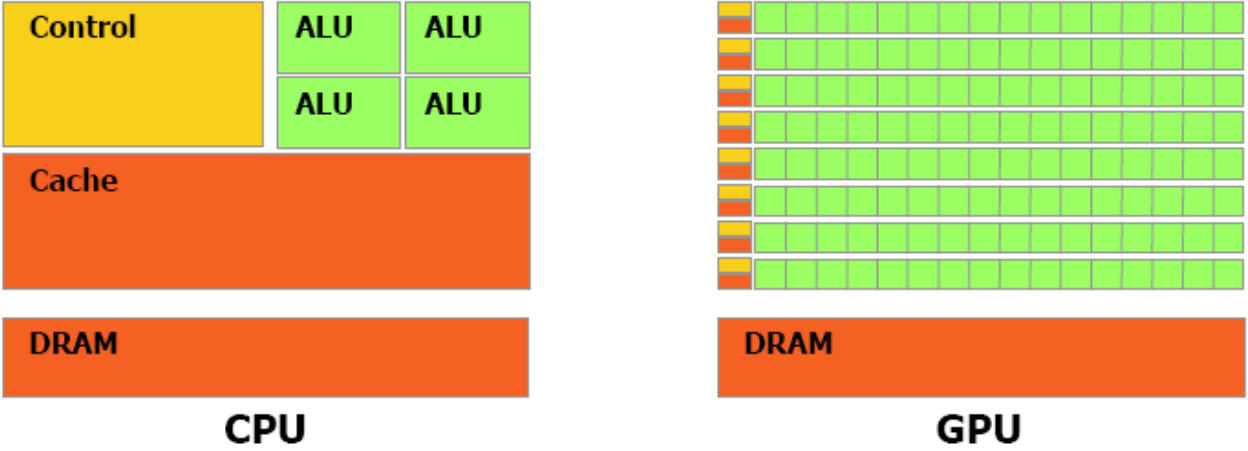
\includegraphics[width = \linewidth]{images/gpu-alu-s}
    \caption{ALUs in CPU vs GPU}
    \label{fig:gpu-alu-s}
\end{figure}

\textbf{Very efficient} for:
\begin{itemize}
    \item Fast Parallel Floating Point Processing
    \item Single Instruction Multiple Data Operations
    \item High Computation per Memory Access
\end{itemize}

\textbf{Not as efficient} for:
\begin{itemize}
    \item Double Precision
    \item Logical Operations on Integer Data
    \item Branching-Intensive Operations
    \item Random Access, Memory-Intensive Operations
\end{itemize}